\documentclass[11pt,letterpaper]{article}
\usepackage[utf8]{inputenc}
\usepackage{fontspec}
\usepackage[margin=1in]{geometry}
\usepackage{graphicx}
\usepackage{pgffor}
\usepackage{amsmath}
\usepackage{amssymb}
\usepackage{fancyhdr}
\usepackage{hyperref}
\usepackage{subcaption}
\usepackage{bbm}
\usepackage{lscape}
\usepackage{ulem}
\usepackage{cancel}
% ------------------------------------------------------

\DeclareMathOperator*{\argmin}{arg\,min}
\DeclareMathOperator*{\argmax}{arg\,max}
\DeclareMathOperator{\Var}{Var}
\DeclareMathOperator{\Cov}{Cov}
\def\inprob{\,{\buildrel p \over \longrightarrow}\,} 
\def\indist{\,{\buildrel d \over \longrightarrow}\,} 

\DeclareMathOperator\F{\mathcal{F}}

% ------------------------------------------------------
 
\usepackage{fontspec}
\usepackage[usenames,dvipsnames]{xcolor}
\usepackage{listings}

%%
%% Julia definition (c) 2014 Jubobs
%%
\lstdefinelanguage{Julia}%
  {morekeywords={abstract,break,case,catch,const,continue,do,else,elseif,%
      end,export,false,for,function,immutable,import,importall,if,in,%
      macro,module,otherwise,quote,return,switch,true,try,type,typealias,%
      using,while,%
      exit,whos,edit,load,is,isa,isequal,typeof,tuple,ntuple,uid,hash,finalizer,convert,promote,
      subtype,typemin,typemax,realmin,realmax,sizeof,eps,promote_type,method_exists,applicable,
      invoke,dlopen,dlsym,system,error,throw,assert,new,Inf,Nan,pi,im,begin,while,for,in,return,
      break,continue,macro,quote,let,if,elseif,else,try,catch,end,bitstype,ccall,do,using,module,
      import,export,importall,baremodule,immutable,local,global,const,Bool,Int,Int8,Int16,Int32,
      Int64,Uint,Uint8,Uint16,Uint32,Uint64,Float32,Float64,Complex64,Complex128,Any,Nothing,None,
      function,type,typealias,abstract},%
   sensitive=true,%
   alsoother={$}, % $
   morecomment=[l]\#,%
   morecomment=[n]{\#=}{=\#},%
   morestring=[s]{"}{"},%
   morestring=[m]{'}{'},%
}[keywords,comments,strings]%

\lstset{%
    language         = Julia,
    basicstyle       = \scriptsize\ttfamily,
    keywordstyle     = \bfseries\color{blue},
    stringstyle      = \color{magenta},
    commentstyle     = \color{ForestGreen},
    numberstyle      = \color{Gray},
    showstringspaces = false,
	showtabs         = false,
	upquote          = false,
    breaklines       = true,
    extendedchars    = true,
}

\begingroup
  \catcode0=12 %
  \makeatletter
  \g@addto@macro\lst@DefEC{%
    \lst@CCECUse\lst@ProcessLetter
   αβγδεϵζηθϑκλμνξπϖρϱσςτυϕφχψωΓΔΘΛΞΠΣΥΦΨΩ∇% *** add Unicode characters ***
    ^^00% end marker
  }%
\endgroup

\setmonofont{Consolas}


\newcommand*{\mathcolor}{}
\def\mathcolor#1#{\mathcoloraux{#1}}
\newcommand*{\mathcoloraux}[3]{%
  \protect\leavevmode
  \begingroup
    \color#1{#2}#3%
  \endgroup
}


% ------------------------------------------------------

\graphicspath{{../plots/pdf/}{../plots/}}
\setlength\parindent{0.0in}

% ------------------------------------------------------

\title{\textbf{Homework 8} \\ Labor Economics}
\author{Mark Agerton and {\color{cyan} Nick Frazier} }
\date{Due Mon, April 13}

% ------------------------------------------------------

\begin{document}

\maketitle

\section{Setup}
Individual knows $\Omega_a = (x_a, y, \epsilon_a)$. His wage is 
\[
    \log w_a^* = \alpha_1 + \alpha_2 x_a + \epsilon_a
\]
We observe
\[
    \log w_a = \log w_a^* + \nu_a
\]
Individual gets per-period payoff
\[
u(\Omega_a) = 
\begin{cases}
    y + \gamma_1 + \gamma_2y         & \text{if } p_a = 0  \text{ (eg, no work)} \\
    y + \exp\{f(x_a) + \epsilon_a\}  & \text{if } p_a = 1  \text{ (eg, work)} 
\end{cases}
\]
Assume iid shocks:
\[
\begin{pmatrix}
\epsilon_a \\ \nu_a
\end{pmatrix}
\sim 
N\left(
0,
\begin{bmatrix}
\sigma_\epsilon^2  & \\
0 & \sigma^2_\nu
\end{bmatrix}
\right)
\]
Objective is
\[
\max_{\{p_a\}_{a=1}^A} \beta^{a-1} E\left[ u(\Omega) \middle| \Omega_a \right]
\]

\section{Recursive formulation}

Write problem recursively for lazy:
\[
V_a^0(x,y,\epsilon_a) = \gamma_1 + (1+\gamma_2)y + \beta E[V_{a+1}( {\color{cyan} x+1},y,\epsilon_{a+1})]
\]
and working:
\[
V_a^1(x,y,\epsilon_a) =
\exp\{f(x_a) + \epsilon_a\} + y + \beta E[V_{a+1}(x+1,y, \epsilon_{a+1})]
\]
Value is
\[
V_a(x,y,\epsilon_a) = \max\left\{V_a^0(x,y,\epsilon_a), V_a^1(x,y,\epsilon_a)\right\}
\]
We normalize the value of afterlife to 0 after assuming earthly actions can't affect it
\[
    V_{A+1}(x,y,\epsilon) = 0
\]
Let $\mathcal W_a$ be the event that we we work, which is 
\[
p_a = 1 \quad \Leftrightarrow \quad
\epsilon_a \geq \underbrace{ \log \bigg( \gamma_1 + \gamma_2 y + E[V_{a+1}^0(x,y)] - E[V_{a+1}^1(x,y)] \bigg) - \alpha_1 - \alpha_2 x_a }_{g(x,y,a)}
\]
Then 
\[
\Pr(\mathcal W_a) = 1- \Phi(g(x,y,a)/\sigma_\epsilon)
\]

\section{Backward induction}

\subsection{Last period}

Last period's value is
\[
V_A(x,y,\epsilon_A) = \max \{ \gamma_1 + \gamma_2 y, \quad \exp(\alpha_1 + \alpha_2 x + \epsilon_A) \} \mathcolor{red}{+ y}
\]
Now
\[
g(x,y,A) = \log(\gamma_1 + \gamma_2 y) - (\alpha_1 + \alpha_2 x)
\]
so 
\[
\Pr(\mathcal W_A) = 1- \Phi\left(\frac{g(x,y,A)}{\sigma_\epsilon} \right) = \pi(x,y,A)
\]
Expected terminal value is
\begin{multline*}
E[V_A(x,y)] = \mathcolor{red}{y +}
    [1-\pi(x,y,A)]\left(\gamma_1 + \gamma_2 y\right)  + \\
    \pi(x,y,A)    \left[\mathcolor{red}{\exp\{\alpha_1 + \alpha_2 x\}} \underbrace{
    \frac{ 1-\Phi\left( \frac{g(x,y,A) - \sigma_\epsilon^2}{\sigma_\epsilon} \right)}
    {\pi(x,y,A)} \exp\{\frac{1}{2}\sigma^2_\epsilon\} }_{E[e^\epsilon_A|\mathcal W^A]} \right]
\end{multline*}
This can be written as
\[
E[V_A(x,y)] = \mathcolor{red}{y} + 
    [1-\pi(x,y,A)]\left[\gamma_1 + \gamma_2 y\right]  + 
    \mathcolor{red}{ \exp\left\{\alpha_1 + \alpha_2 x + \frac{\sigma_\epsilon^2}{2}\right\}}
    \left[1-\Phi\left( \frac{g(x,y,A) - \sigma_\epsilon^2}{\sigma_\epsilon} \right)\right] 
\]

\subsection{Other periods}
This means
\[
    g(x,y,a) = \log \bigg( \gamma_1 + \gamma_2 y + \beta\overbrace{E[V_{a+1}^0(x,y)] - E[V_{a+1}^1(x,y)]}^{\Delta EV(x,y,a)} \bigg) - \alpha_1 - \alpha_2 x_a 
\]
and
\[
\mathcal W_a = \left\{\epsilon_a \geq g(x,y,a) \right\}
\]
so
\[
\Pr(\mathcal W_a) = 1- \Phi\left(\frac{g(x,y,a)}{\sigma_\epsilon} \right) = \pi(x,y,a)
\]
and
\begin{align*}
E[V_a(x,y)] 
&= \mathcolor{red}{y}  
+ [1-\pi(x,y,a)]\left\{\gamma_1 + \gamma_2 y + E[V_{a+1}(x,y)] \right\}  \\ 
&+ \pi(x,y,a)E[V_{a+1}(x+1,y)] + \mathcolor{red}{ \exp\left\{\alpha_1 + \alpha_2 x + \frac{\sigma_\epsilon^2}{2}\right\}}
    \left[1-\Phi\left( \frac{g(x,y,a) - \sigma_\epsilon^2}{\sigma_\epsilon} \right)\right] 
\end{align*}
Note that we could simply use the general definition for $V_a$ and $g(x,y,a)$ and specify $V_{A+1} = 0$. This would be a bit neater (ie, for each agent, have $A+1$ periods and just say $V_{A+1} = 0$... then start recursion at $a=A$.  

\section{Estimation}

We have states $\Omega_{ia} = (x,y,a,\epsilon)_{ia}$ and control $p_{ia} \in \{0,1\}$. 

Immediately we can get parameters governing distribution of non-labor income from a kernel density estimation of observed $y_i$ values. Or, since we know if we know the underlying distribution we just need $\mu_y$ and $\sigma_y$ which can be estimated by $N^{-1}\sum\nolimits_i y_i$ and $\widehat{SE(y_i)}$. Number of periods is irrelevant and are consistent as $N\rightarrow \infty$. .

Remaining parameters are
\[
\theta = \{ \alpha_1, \alpha_2, \gamma_1, \gamma_2, \sigma_\epsilon^2, \sigma^2_\nu \}
\]
We'll need functions(?) or matrices of(?)
\[
V_a^0(x,y) \quad V_a^1(x,y) \quad g(x,y,a) \quad \pi(x,y,a) \quad w(x,\epsilon; \alpha_1, \alpha_2)
\]
Note that $g(x,y,a)$ is a function of $a$ because it has $\Delta E[V_{a+1}(x,y)]$

\subsection{Plan}
\begin{enumerate}
    \item Given $\theta$, calculate functions {\color{cyan} I think we are just starting at $t=A$ here and so $\Delta E[V_{a+1}(x,y)] = 0$ and we do not need to fix a $\theta$. Can recover $g$ without.}
    \item Run probit for working in $A$
    \item Estimate wages as 
    \[
        \log w = \underbrace{\alpha_1 + \alpha_2 x + \sigma_\epsilon \lambda(y,x,a)}_{E[\log w_a^* | \mathcal W_a]} + \nu
    \] 
    where
    \[
        \lambda(x,y,a) = E\left[\frac{\epsilon}{\sigma} \middle | \frac{\epsilon}{\sigma} \underbrace{\geq}_{\text{notes were } \leq} \frac{g(x,y,a)}{\sigma_\epsilon}\right]
        = \frac{\phi(g/\sigma)}{1- \Phi(g/\sigma)}
    \]
    \item Compute $\Delta E[V_A(x,y)]$
    \item Run probit for $A-1$...
\end{enumerate}

\section{Results}

\lstinputlisting[frame=single, caption=Functions used]{../code/parameterization_keep.jl} \\


		{
		\vspace{-1.5cm}
		\centering
		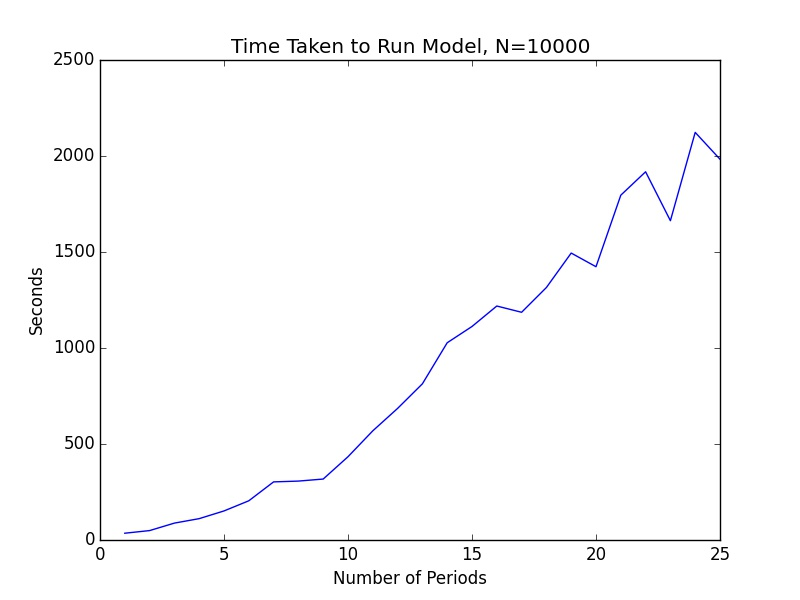
\includegraphics[width=\textwidth]{time_taken_keep.jpg} \\
		}

\subsection{Sample Output}

\lstinputlisting[frame=single, caption=Functions used]{../code/output_keep.jl}



\end{document}
